% 2011 年江苏卷第 18 题：椭圆 x^2/4 + y^2/2 = 1 与点 M,N,P,A,B,C。
% 来源 PDF：普通高考/2011/2011江苏.pdf，SHA-256 71763ef5d0c2b5800c12515e6b3addb77e585b2460fd11c1013fcec6f050ece9。
% 原页：第 1 页第 3 栏下部，书页码 675。按题设取 k=1 示意。
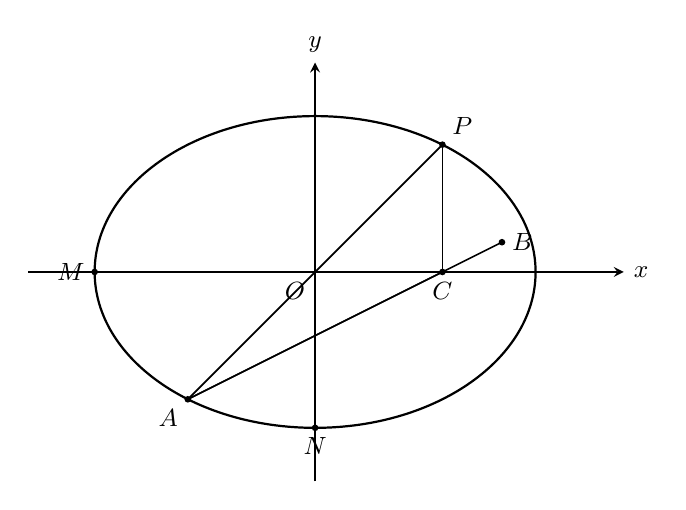
\begin{tikzpicture}[>=stealth, semithick, font=\small, x=1.4cm, y=1.4cm]
  \draw[->] (-2.6,0) -- (2.8,0) node[right] {$x$};
  \draw[->] (0,-1.9) -- (0,1.9) node[above] {$y$};
  \node[below left] at (0,0) {$O$};
  \draw[thick] (0,0) ellipse ({2} and {1.414});
  \coordinate (O) at (0,0);
  \coordinate (M) at (-2,0);
  \coordinate (N) at (0,-1.414);
  \coordinate (P) at (1.155,1.155);
  \coordinate (C) at (1.155,0);
  \coordinate (A) at (-1.155,-1.155);
  \coordinate (B) at (1.695,0.270);
  \draw (P)--(O)--(A);
  \draw (P)--(C);
  \draw (A)--(B);
  \draw (A)--(C);
  \fill (M) circle (1.2pt) node[left] {$M$};
  \fill (N) circle (1.2pt) node[below] {$N$};
  \fill (P) circle (1.2pt) node[above right] {$P$};
  \fill (A) circle (1.2pt) node[below left] {$A$};
  \fill (B) circle (1.2pt) node[right] {$B$};
  \fill (C) circle (1.2pt) node[below] {$C$};
\end{tikzpicture}
